\section{Risk and Technical Debt}

To measure the risks of this project we will use the following 3x3 risk matrix, which will help us develop the 
\gls{risk assessment}:

\begin{figure}[H]
    \centering
    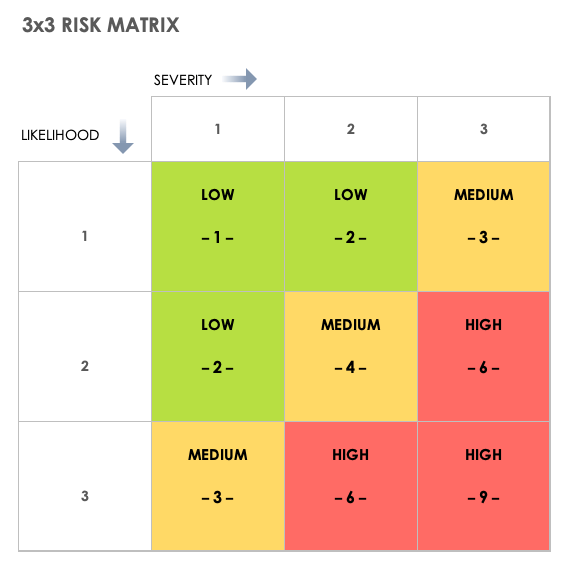
\includegraphics[width=0.5\textwidth]{assets/Risk-Matrix.png}
    \caption{3x3 Risk Matrix Template\\ Source: \citet{refonline:smtrisk}  }
    \label{fig:risk_matrix_template}
\end{figure}

On the left side we see the risk table  defined after several discussion with the team members.
On the right side there are the elements to which the table refers to:

\begin{table}[H]
	\begin{minipage}{0.5\linewidth}
		\label{table:student}
		\centering
        \resizebox{7cm}{!}{%
        \begin{tabular}{|l|l|l|l|l|l|l|}
            \toprule
            \multicolumn{1}{c}{\multirow{2}{*}{\textbf{Risk Criteria}}} & \multicolumn{6}{c}{\textbf{Element ID}} \\ 
            %\midrule
            \multicolumn{1}{c}{}            & \multicolumn{1}{c}{\textbf{1}} & \multicolumn{1}{c}{\textbf{2}} & \multicolumn{1}{c}{\textbf{3}} & \multicolumn{1}{c}{\textbf{4}} & \multicolumn{1}{c}{\textbf{5}} & \multicolumn{1}{c}{\textbf{6}} \\ \hline
            \textbf{Unproven technology}      & {\cellcolor{green} 1} & {\cellcolor{green} 1} & {\cellcolor{green} 1} & {\cellcolor{green} 1} & {\cellcolor{green} 1} & {\cellcolor{green} 1} \\ \hline
            \textbf{Performance}              & {\cellcolor{green} 2} & {\cellcolor{green} 2} & {\cellcolor{green} 1} & {\cellcolor{green} 1} & {\cellcolor{green} 1} & {\cellcolor{green} 1} \\ \hline
            \textbf{Scalability}              & {\cellcolor{green} 1} & {\cellcolor{green} 1} & {\cellcolor{green} 2} & {\cellcolor{green} 1} & {\cellcolor{green} 1} & {\cellcolor{green} 1} \\ \hline
            \textbf{Availability}             & {\cellcolor{green} 1} & {\cellcolor{green} 1} & {\cellcolor{yellow} 4} & {\cellcolor{green} 2} & {\cellcolor{green} 1} & {\cellcolor{green} 1} \\ \hline
            \textbf{Data loss}                & {\cellcolor{green} 1} & {\cellcolor{green} 1} & {\cellcolor{yellow} 3} & {\cellcolor{green} 1} & {\cellcolor{green} 1} & {\cellcolor{green} 1} \\ \hline
            \textbf{Single points of failure} & {\cellcolor{green} 1} & {\cellcolor{green} 1} & {\cellcolor{yellow} 4} & {\cellcolor{yellow} 4} & {\cellcolor{green} 1} & {\cellcolor{green} 1} \\ \hline
            \textbf{Security}                 & {\cellcolor{green} 1} & {\cellcolor{green} 2} & {\cellcolor{yellow} 3} & {\cellcolor{green} 2} & {\cellcolor{green} 2} & {\cellcolor{green} 2} \\ \hline
            %\bottomrule
        \end{tabular}%
        }
	\end{minipage}\hfill
	\begin{minipage}{0.45\linewidth}
		\centering
		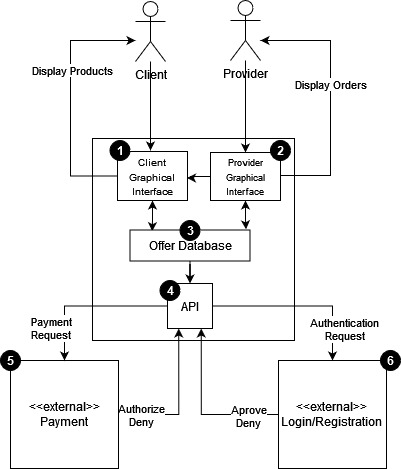
\includegraphics[width=6cm]{assets/risk_technical_context.jpg}
		\captionof{figure}{Modified from Figure \ref{fig:technical_context}}
		\label{ }
	\end{minipage}
\end{table}


% backup figure with numbers
% \begin{figure}[H]
%     \centering
%     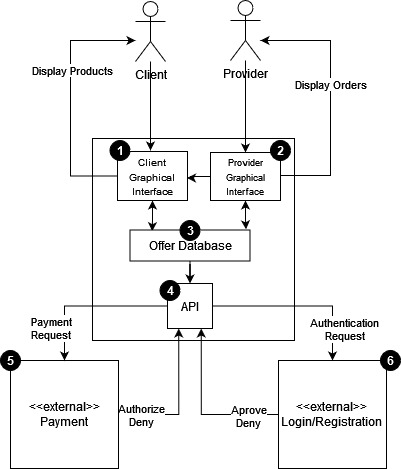
\includegraphics[width=0.4\textwidth]{assets/risk_technical_context.jpg}
%     \caption{Modified from Figure \ref{fig:technical_context}}
%     \label{fig:risk_technical_context}
% \end{figure}

% backup
% \begin{table}[H]
%     \centering
%     \resizebox{7cm}{!}{%
%     \begin{tabular}{|l|l|l|l|l|l|l|}
%     \toprule
%     \multicolumn{1}{c}{\multirow{2}{*}{\textbf{Risk Criteria}}} & \multicolumn{6}{c}{\textbf{Element ID}} \\ 
%     %\midrule
%     \multicolumn{1}{c}{}            & \multicolumn{1}{c}{\textbf{1}} & \multicolumn{1}{c}{\textbf{2}} & \multicolumn{1}{c}{\textbf{3}} & \multicolumn{1}{c}{\textbf{4}} & \multicolumn{1}{c}{\textbf{5}} & \multicolumn{1}{c}{\textbf{6}} \\ \hline
%     \textbf{Unproven technology}      & {\cellcolor{green} 1} & {\cellcolor{green} 1} & {\cellcolor{green} 1} & {\cellcolor{green} 1} & {\cellcolor{green} 1} & {\cellcolor{green} 1} \\ \hline
%     \textbf{Performance}              & {\cellcolor{green} 2} & {\cellcolor{green} 2} & {\cellcolor{green} 1} & {\cellcolor{green} 1} & {\cellcolor{green} 1} & {\cellcolor{green} 1} \\ \hline
%     \textbf{Scalability}              & {\cellcolor{green} 1} & {\cellcolor{green} 1} & {\cellcolor{green} 2} & {\cellcolor{green} 1} & {\cellcolor{green} 1} & {\cellcolor{green} 1} \\ \hline
%     \textbf{Availability}             & {\cellcolor{green} 1} & {\cellcolor{green} 1} & {\cellcolor{yellow} 4} & {\cellcolor{green} 2} & {\cellcolor{green} 1} & {\cellcolor{green} 1} \\ \hline
%     \textbf{Data loss}                & {\cellcolor{green} 1} & {\cellcolor{green} 1} & {\cellcolor{yellow} 3} & {\cellcolor{green} 1} & {\cellcolor{green} 1} & {\cellcolor{green} 1} \\ \hline
%     \textbf{Single points of failure} & {\cellcolor{green} 1} & {\cellcolor{green} 1} & {\cellcolor{yellow} 4} & {\cellcolor{yellow} 4} & {\cellcolor{green} 1} & {\cellcolor{green} 1} \\ \hline
%     \textbf{Security}                 & {\cellcolor{green} 1} & {\cellcolor{green} 2} & {\cellcolor{yellow} 3} & {\cellcolor{green} 2} & {\cellcolor{green} 2} & {\cellcolor{green} 2} \\ \hline
%     %\bottomrule
% \end{tabular}%
%     }
% \end{table}


\subsection{Motivation}

\begin{table}[H]
    \setstretch{1.0}
        \begin{tabularx}{\textwidth}{|c|X|X|X|}
        \toprule
           \textbf{Risk Criteria} & \textbf{1 Client Graphical Interface} & \textbf{2 Provider Graphical Interface} & \textbf{3 Offer Database} \\
        \midrule
        \textbf{Unproven technology}& \textit{not applicable} & \textit{not applicable} & \textit{not applicable} \\
        \hline
        \textbf{Performance} & Concerns regarding a such dynamic shop. Data displayed & Concerns regarding a such dynamic shop. Data update. & \textit{not applicable} \\
        \hline
        \textbf{Scalability} & \textit{not applicable} & \textit{not applicable} & One database can be overwhelmed if the number of user is not limited for this prototype version. \\
        \hline
        \textbf{Availability} & \textit{not applicable} & \textit{not applicable} & In case of intense traffic the latency can be more than expected. \\
        \hline
        \textbf{Data loss} & \textit{not applicable} & \textit{not applicable} & Nowadays no company can survive in case of data loss. Technical damages can be 
        mostly easy fixed, but moral damage stays forever. \\
        \hline
        \textbf{Single points of failure} & \textit{not applicable} & \textit{not applicable} & Only one component gives always this risk. Increasing the 
        number of components increases also the total development costs \\
        \hline
        \textbf{Security} & \textit{not applicable} the client's input is always processed
        by the \glsplural{API} and by the third party providers & If no strong data filtering exists, providers can upload
        malicious files or execute unwished commands. & The filtering of the input should occur mostly on the server side, Source
        no external access can figure out, how it is implemented. \\
        \bottomrule
    \end{tabularx}
\end{table}

\begin{table}[H]
    \setstretch{1.0}
    \begin{tabularx}{\textwidth}{|c|X|X|X|}
        \toprule
        \textbf{Risk Criteria} & \textbf{4 \gls{API}} & \textbf{5 External Payment Service} & \textbf{6 External Authentication Service} \\
        \midrule
        \textbf{Unproven technology} & \textit{not applicable} & \textit{not applicable}  & \textit{not applicable}  \\
        \hline
        \textbf{Performance} & \textit{not applicable} & \textit{not applicable}  & \textit{not applicable} \\
        \hline
        \textbf{Scalability} & \textit{not applicable} & \textit{not applicable} & \textit{not applicable} \\
        \hline
        \textbf{Availability} & The access to the products become unstable. & \textit{not applicable} & \textit{not applicable} \\
        \hline
        \textbf{Data loss} & \textit{not applicable} & \textit{not applicable} & \textit{not applicable} \\
        \hline
        \textbf{Single points of failure} & In case of failure login, registration and payment are compromised. & \textit{not applicable} & \textit{not applicable} \\
        \hline
        \textbf{Security} & Lack of practical experience within the team about this topic. we rely on the service provided by the third party companies 
        & \gls{SLA} Less than 99.5\% but equal to or greater than 95.0\% \cite{refmisc:paycSLA} & \gls{SLA} < 99.99\% - >= 99.9\% \cite{refmisc:auth0sla}	\\
        \bottomrule
    \end{tabularx}
\end{table}
%1 - 
%